% ============================================================
% ============================================================
%  CONVECTIVE HEAT TRANSFER & THERMODYNAMICS
% ============================================================
% ============================================================

\section[HTC \& Thermodynamic]{\textbf{Convective Heat Transfer \& Thermodynamics}}


% ============================================================
%  HTC Distributions
% ============================================================

\begin{frame}{\small  Convective Heat-Transfer Coefficient (L1)}
\scriptsize

\vspace{-0.3cm}
% ------------------------------------------------------------
% Standard HTC comparison
% ------------------------------------------------------------
\only<1>{
\begin{columns}[T,onlytextwidth]

\begin{column}{0.50\textwidth}
    \centering
    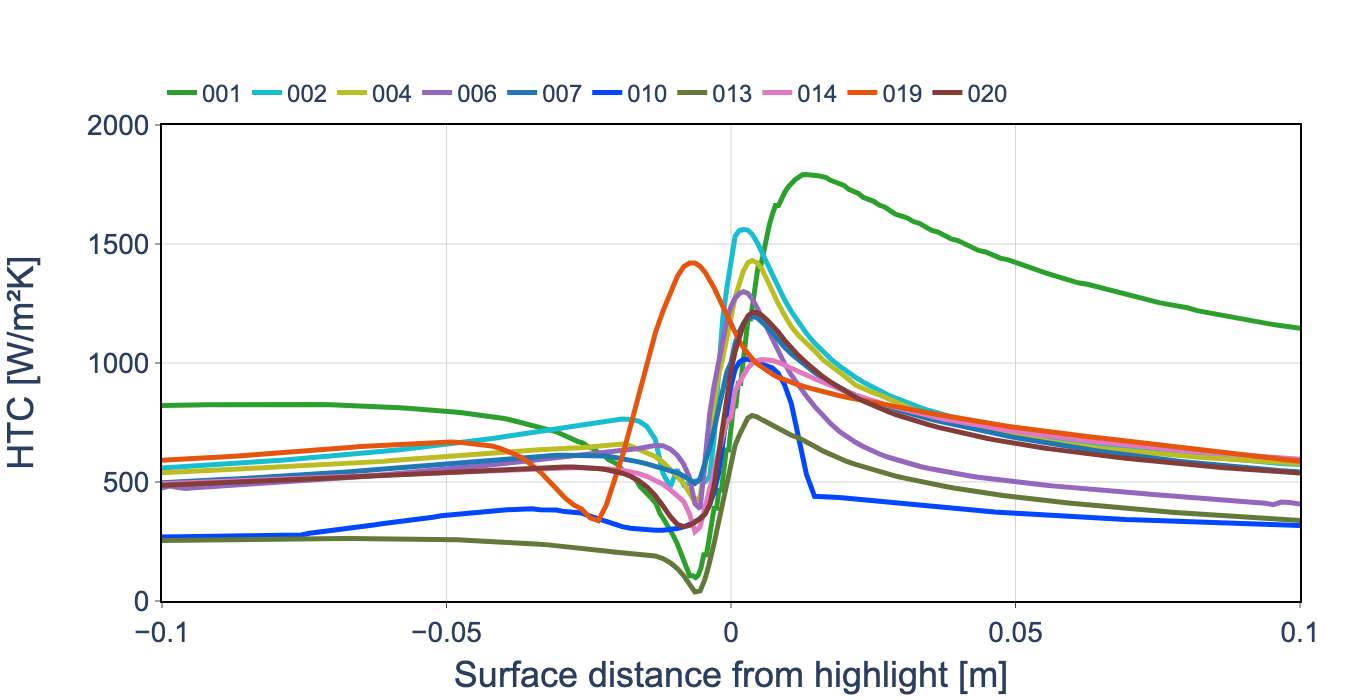
\includegraphics[trim={0cm 0cm 1cm 2.6cm}, clip, width=\textwidth]{FIGURES/HTC/tc_naca0012_ae3932_L1_htc_vs_s_slice_0p9144_all_roughness.png}
    {\scriptsize\textbf{AE3932}}
\end{column}

\begin{column}{0.50\textwidth}
    \centering
    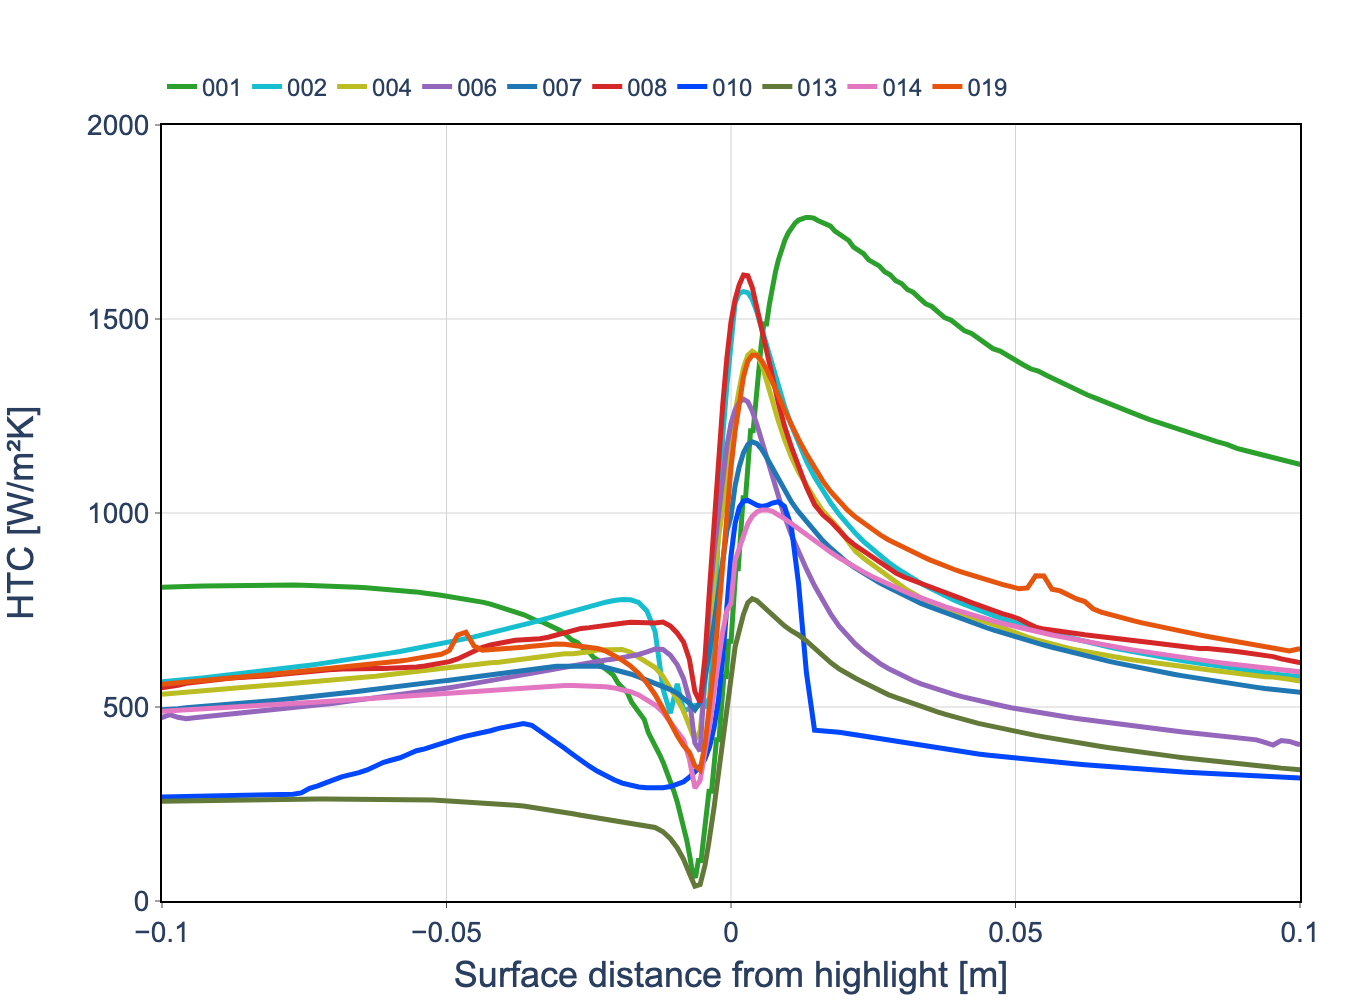
\includegraphics[trim={0cm 0cm 1cm 2.6cm}, clip, width=\textwidth]{FIGURES/HTC/tc_naca0012_ae3933_L1_htc_vs_s_slice_0p9144_all_roughness.png}
    {\scriptsize\textbf{AE3933}}
\end{column}

\end{columns}
}

% ------------------------------------------------------------
% HTC grouped by roughness
% ------------------------------------------------------------
\only<2>{
\begin{columns}[T,onlytextwidth]
\begin{column}{0.50\textwidth}
    \centering
    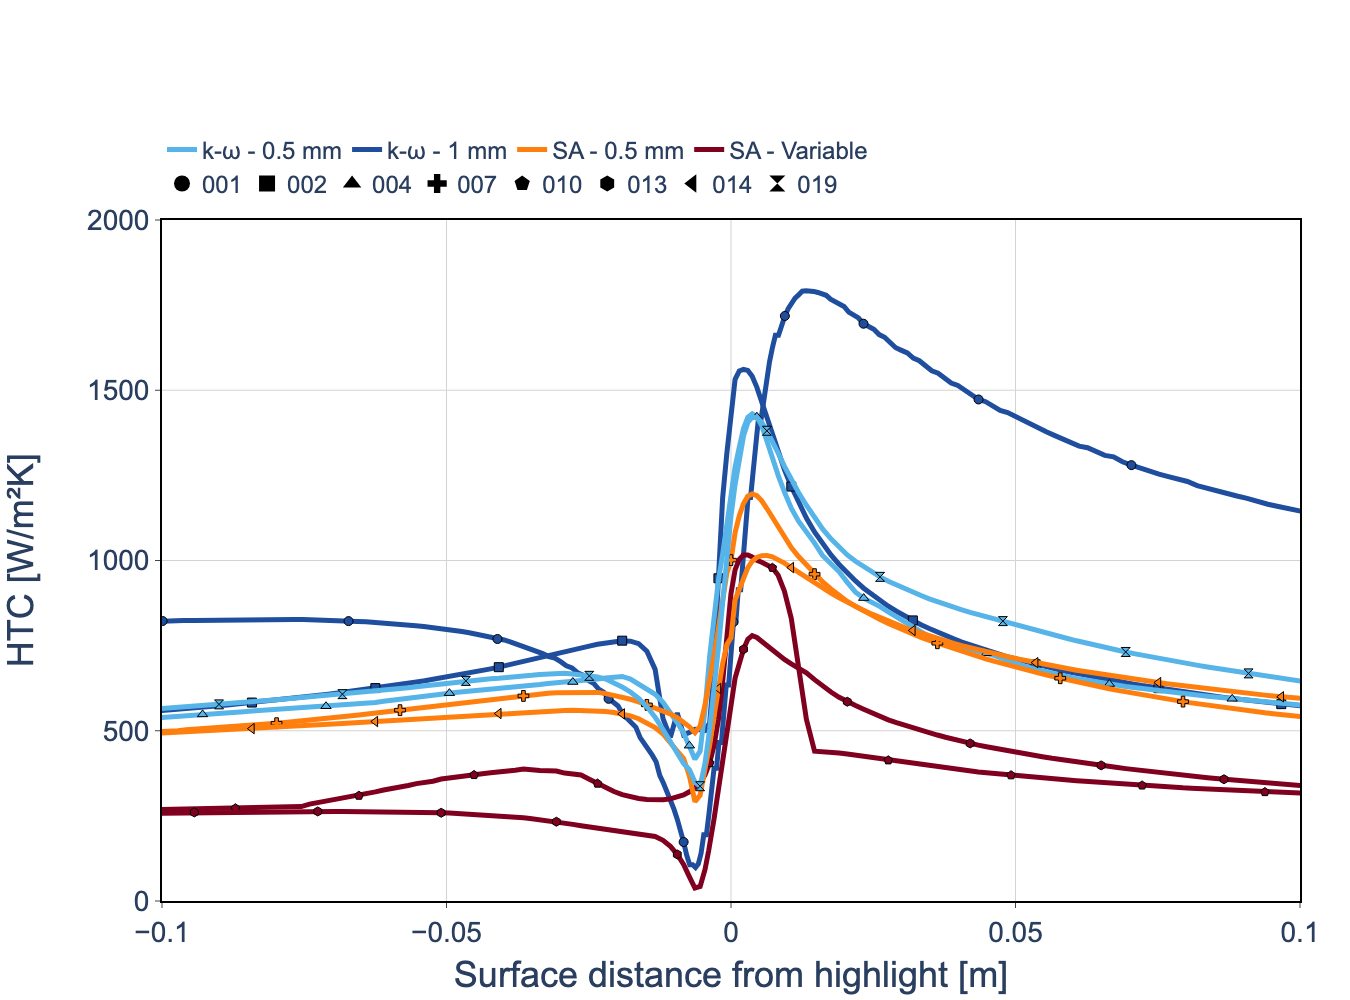
\includegraphics[trim={0cm 0cm 1cm 3.8cm}, clip, width=\textwidth]{FIGURES/HTC/tc_naca0012_ae3932_L1_htc_vs_s_slice_0p9144_grouped_turbulence_models.png}
    {\scriptsize\textbf{AE3932}}
\end{column}

\begin{column}{0.50\textwidth}
    \centering
    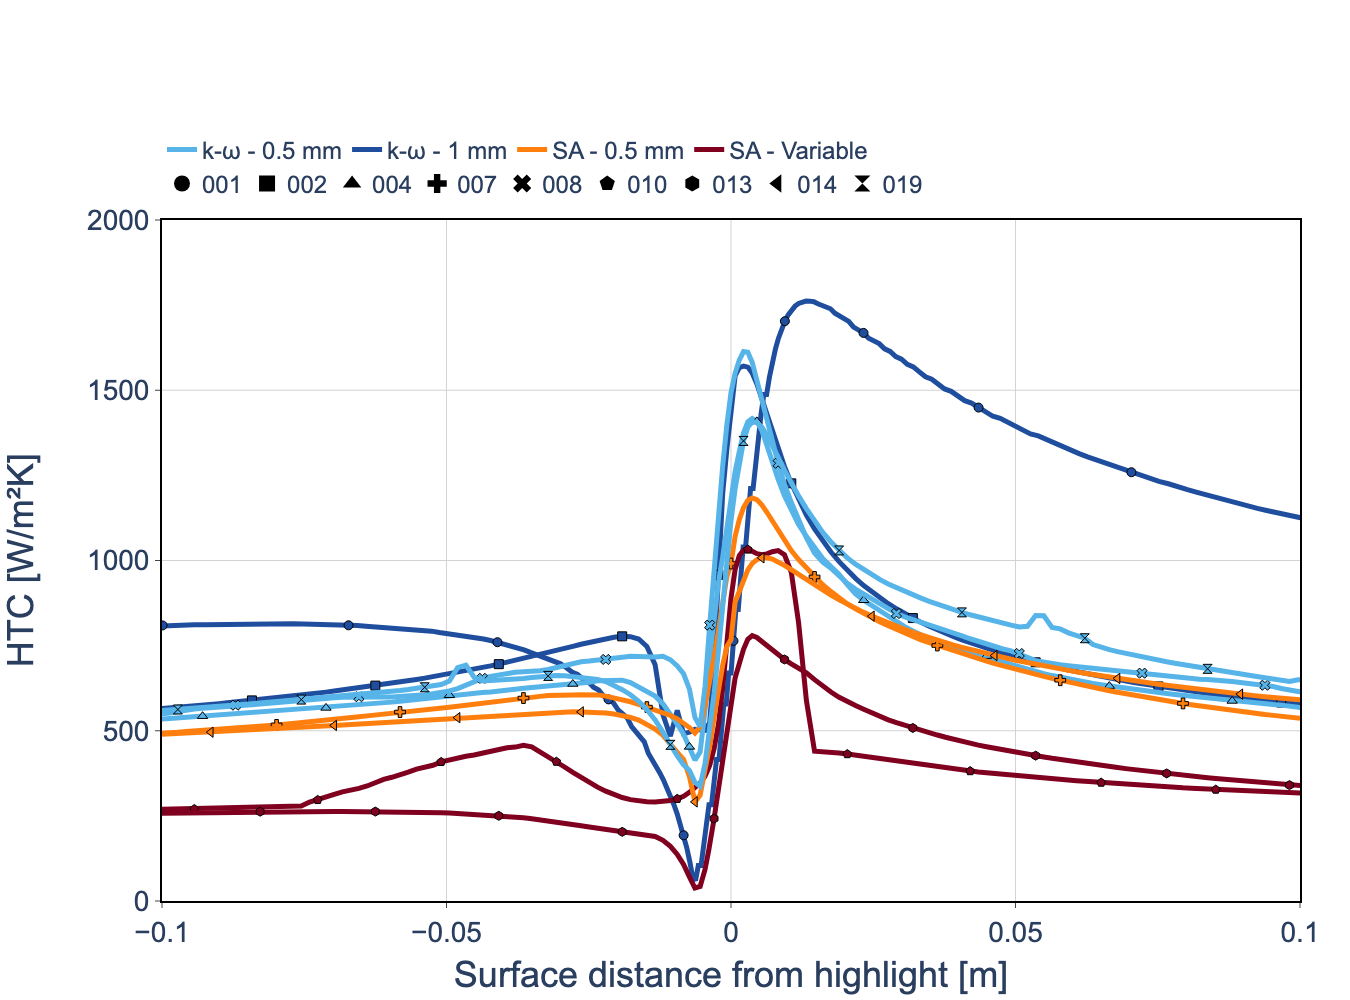
\includegraphics[trim={0cm 0cm 1cm 3.8cm}, clip, width=\textwidth]{FIGURES/HTC/tc_naca0012_ae3933_L1_htc_vs_s_slice_0p9144_grouped_turbulence_models.png}
    {\scriptsize\textbf{AE3933}}
\end{column}
\end{columns}

\vspace{-0.05cm}
\centering
\textbf{Grouped by Turbulence Model / Roughness}

\vspace{0.1cm}
{\tiny\centering
\textit{Note: Colors indicate Turbulence Model / Roughness groups and are not associated with participant IDs.}
\par}
}

\vspace{-0.15cm}

\begin{block}{\scriptsize Observations}
\begin{itemize}
    \item<1-> Significant $HTC$ code-to-code variability is observed, particularly near the leading edge.
    \item<2-> Turbulence modeling and roughness height appear to be primary contributors to the spread, while differences in $HTC$ computation methodology also play a role.
\end{itemize}
\end{block}
\end{frame}


% ============================================================
%  Integrated Convective Heat Transfer
% ============================================================

\begin{frame}[shrink=15]{\small  Integrated Convective Heat Transfer}
\scriptsize

\centering
\vspace{-0.1cm}
\begin{minipage}{0.90\textwidth}
\begin{block}{\scriptsize Grid-Convergence Metric}
To assess whether the differences in the local $HTC$ distributions translate
into a clear grid-convergence behavior, an integrated convective heat-transfer
quantity is evaluated along the surface slice:
\[
\boxed{
Q_c'
=
\int
HTC(s)
\left[
T_s(s)-T_{\mathrm{rec}}(s)
\right]\,ds
}
\qquad
[Q_c'] = \mathrm{W/m}.
\]

The submitted $HTC$ and surface temperature $T_s$ are used directly.
The recovery temperature $T_{\mathrm{rec}}$, however, was not part of the
submitted dataset and must therefore be reconstructed.
\end{block}
\end{minipage}

\vspace{0.15cm}

\begin{minipage}{0.90\textwidth}
\begin{block}{\scriptsize Recovery Temperature Reconstruction}
The submitted pressure coefficient is used to estimate the local external-flow
state and subsequently the recovery temperature:
\[
\boxed{
C_p(s)
\;\longrightarrow\;
p_e(s)
\;\longrightarrow\;
M_e(s)
\;\longrightarrow\;
T_e(s)
\;\longrightarrow\;
T_{\mathrm{rec}}(s)
}
\]

Assuming $p_s \simeq p_e$ and an isentropic external flow,
\[
\frac{p_e}{p_\infty}
=
1+\frac{\gamma}{2}M_\infty^2 C_{p,e},
\qquad
M_e^2
=
\frac{2}{\gamma-1}
\left[
\left(\frac{p_0}{p_e}\right)^{(\gamma-1)/\gamma}-1
\right],
\]
\[
T_e
=
\frac{T_0}
{1+\dfrac{\gamma-1}{2}M_e^2},
\qquad
T_{\mathrm{rec}}
=
T_e
\left[
1+r\frac{\gamma-1}{2}M_e^2
\right],
\qquad
r=Pr^{1/3}\approx0.9.
\]

\end{block}
\end{minipage}

\end{frame}


% ============================================================
%  Recovery Temperature
% ============================================================

\begin{frame}{\small  Reconstructed Recovery Temperature (L1)}
\scriptsize

\centering
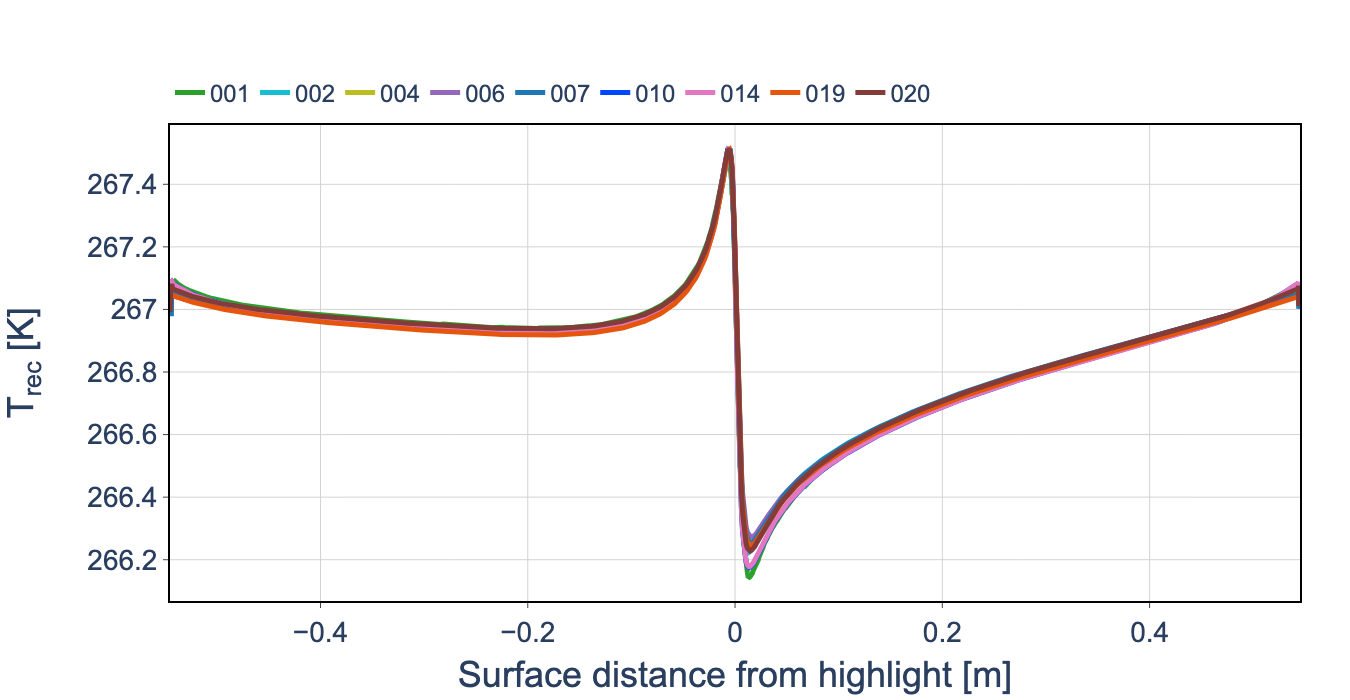
\includegraphics[trim={0cm 0cm 1cm 2.6cm}, clip, width=0.5\textwidth]{FIGURES/HTC/tc_naca0012_ae3932_L1_recovery_temperature_vs_s_slice_0p9144_all_roughness.png}

{\scriptsize\textbf{$\boldsymbol{T_{rec}}$ vs s}}

\vspace{-0.15cm}

\begin{block}{\scriptsize Observations}
\begin{itemize}
    \item $T_{\mathrm{rec}}$ is closely clustered, consistent with the agreement in $C_p$.
    \item Variability in $Q_c'$ therefore will originate primarily from $HTC$ and $T_s$.
\end{itemize}
\end{block}

\end{frame}


% ============================================================
%  Convective Heat Transfer Grid Convergence
% ============================================================

\begin{frame}{\small  Integrated Convective Heat Transfer Grid Convergence}
\scriptsize

\vspace{-0.15cm}
% ------------------------------------------------------------
% Standard Qc' comparison
% ------------------------------------------------------------
\only<1>{
\begin{columns}[T,onlytextwidth]

\begin{column}{0.50\textwidth}
    \centering
    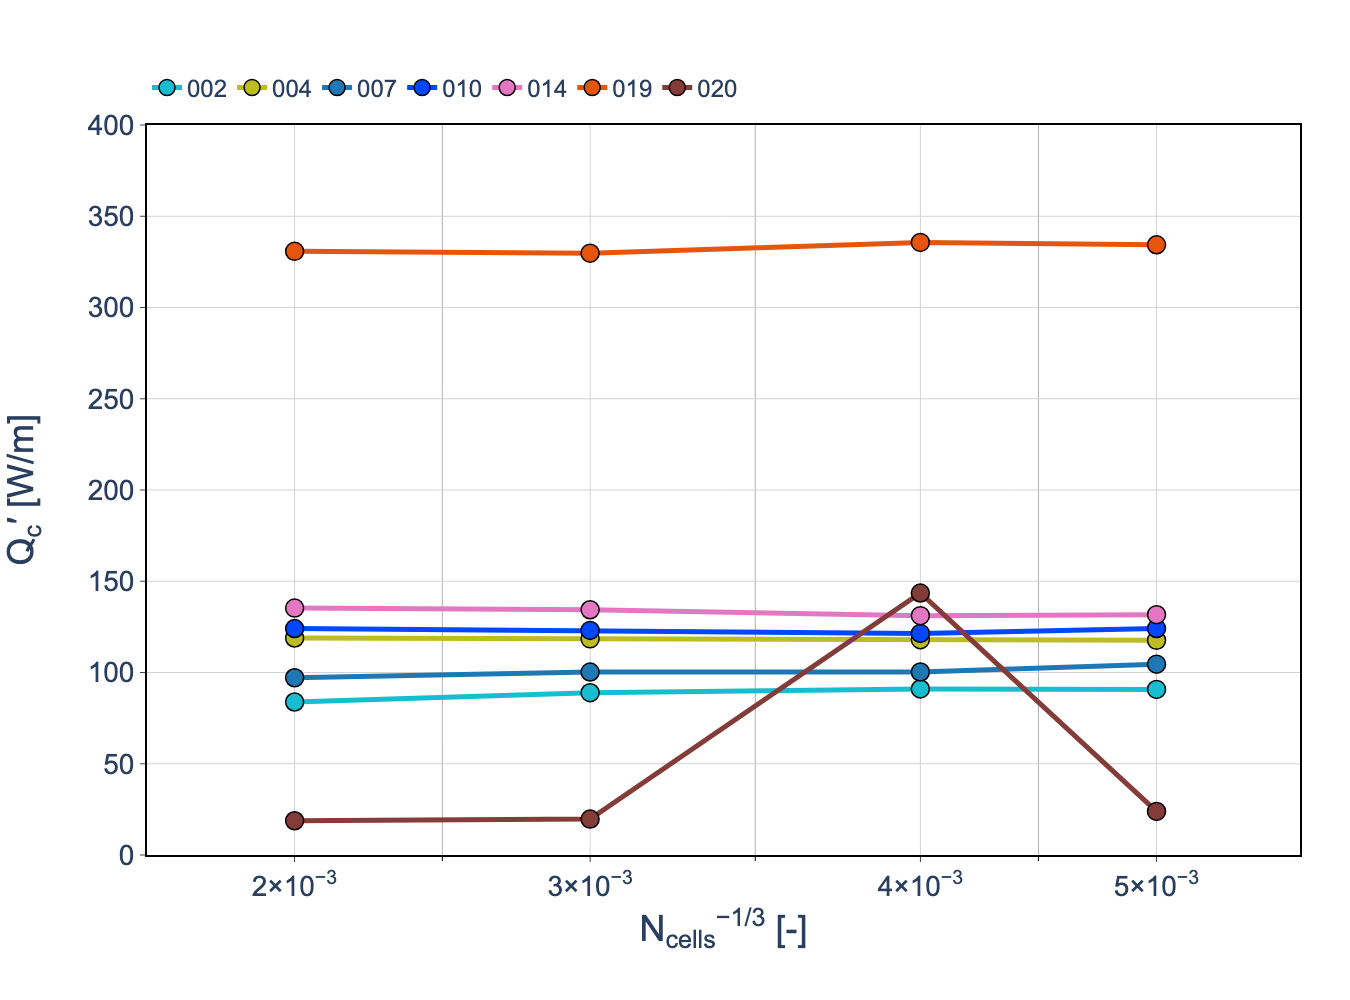
\includegraphics[trim={0cm 1cm 1cm 2.6cm}, clip, width=0.98\textwidth]{FIGURES/HTC/tc_naca0012_ae3932_qc_prime_vs_n_y_0.9144.png}
    \textbf{AE3932}
\end{column}

\begin{column}{0.50\textwidth}
    \centering
    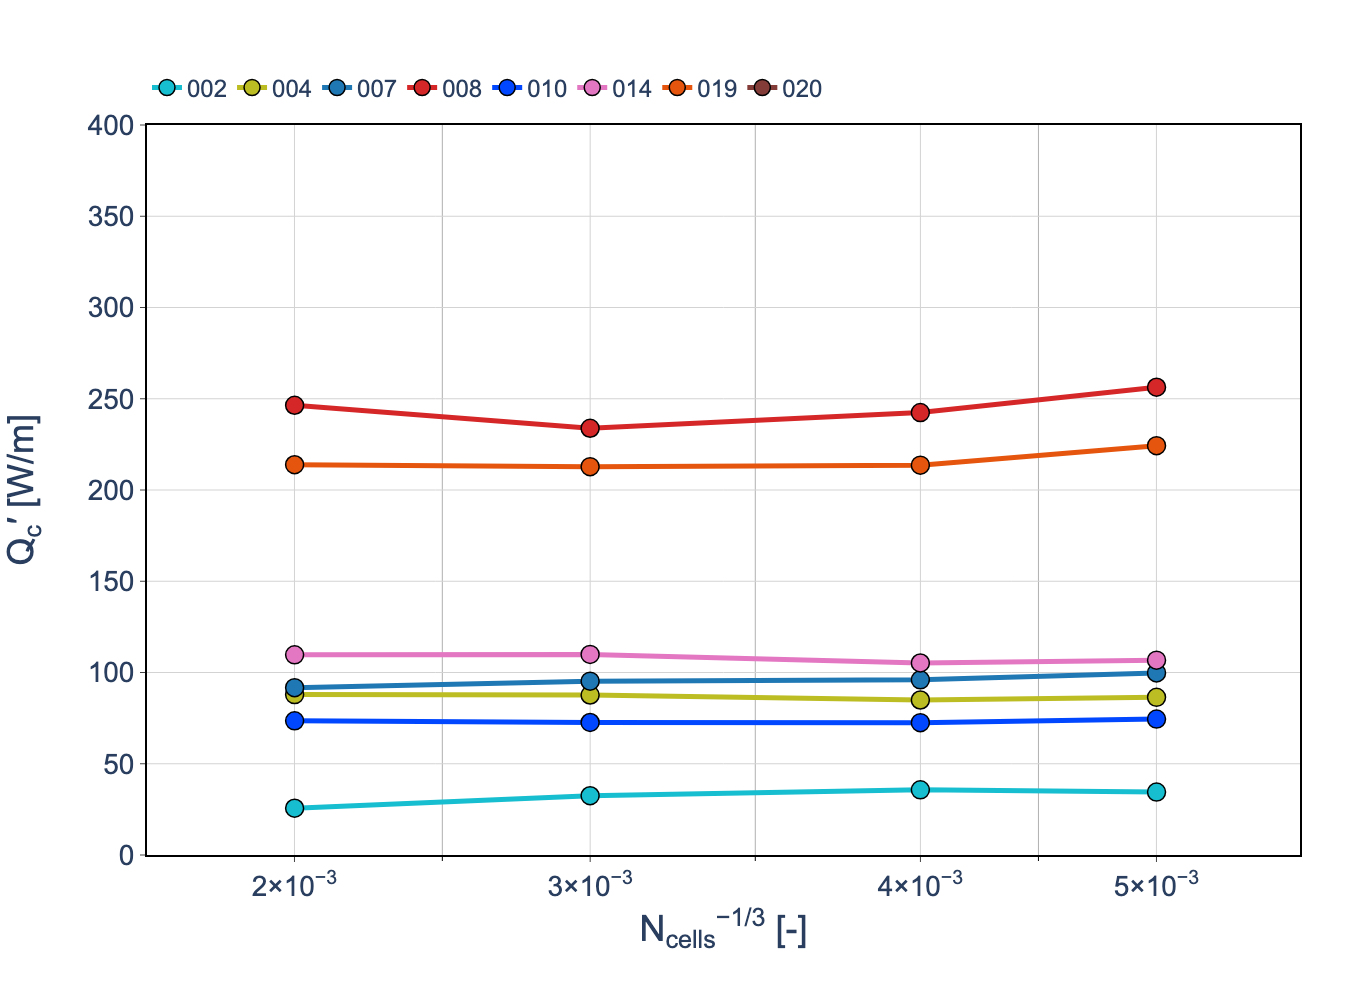
\includegraphics[trim={0cm 1cm 1cm 2.6cm}, clip, width=0.98\textwidth]{FIGURES/HTC/tc_naca0012_ae3933_qc_prime_vs_n_y_0.9144.png}
    \textbf{AE3933}
\end{column}

\end{columns}
}

% ------------------------------------------------------------
% Qc' grouped by roughness
% ------------------------------------------------------------
\only<2>{
\begin{columns}[T,onlytextwidth]

\begin{column}{0.50\textwidth}
    \centering
    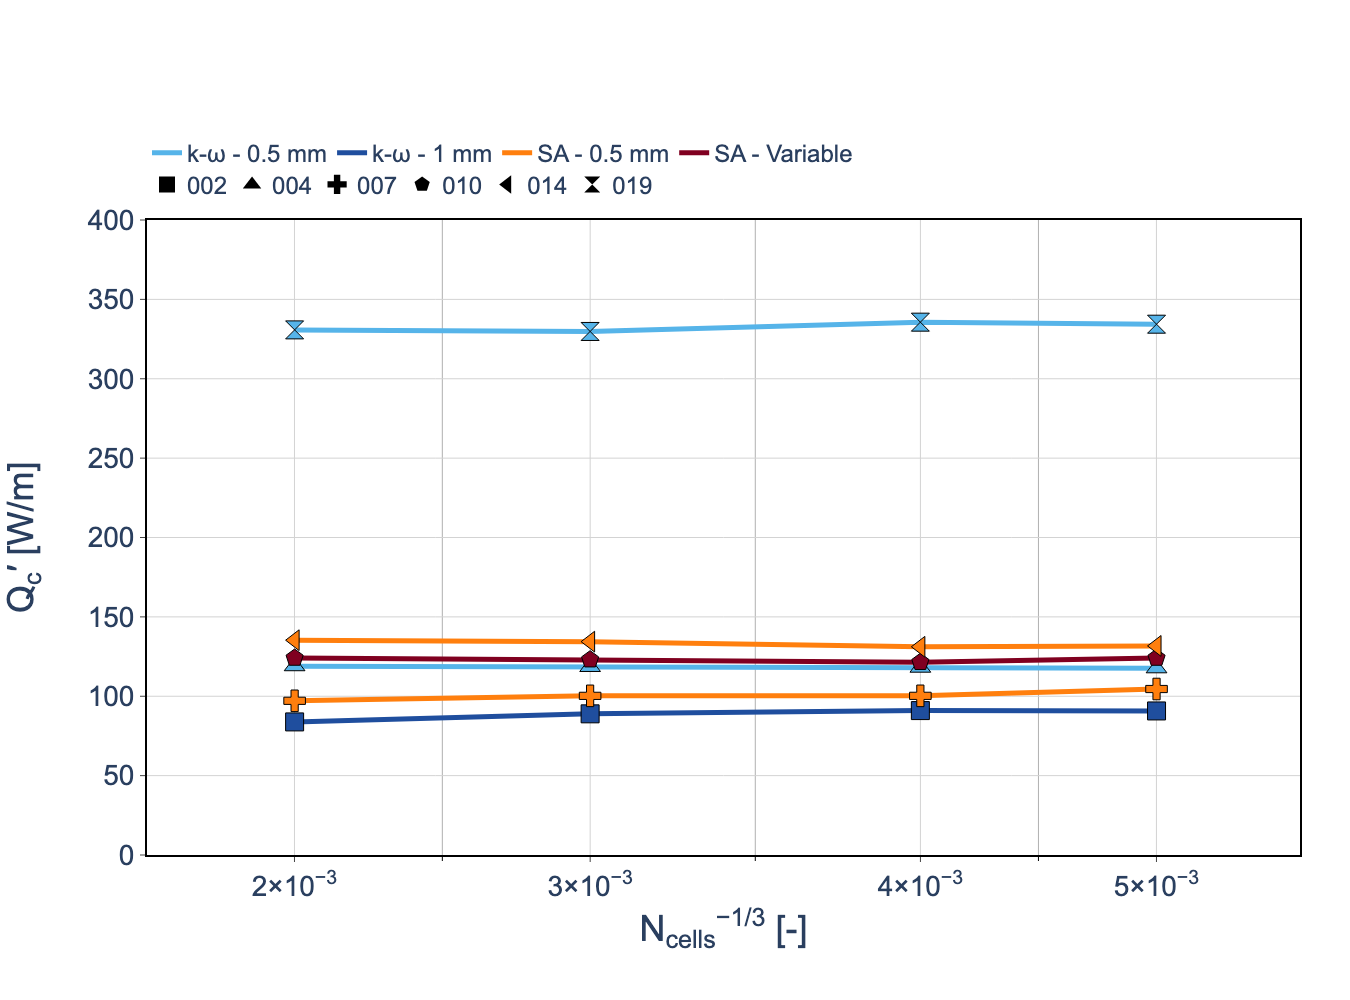
\includegraphics[trim={0cm 1cm 1cm 2.6cm}, clip, width=0.98\textwidth]{FIGURES/HTC/tc_naca0012_ae3932_qc_prime_vs_n_y_0.9144_grouped_turbulence_models.png}
    \textbf{AE3932}
\end{column}

\begin{column}{0.50\textwidth}
    \centering
    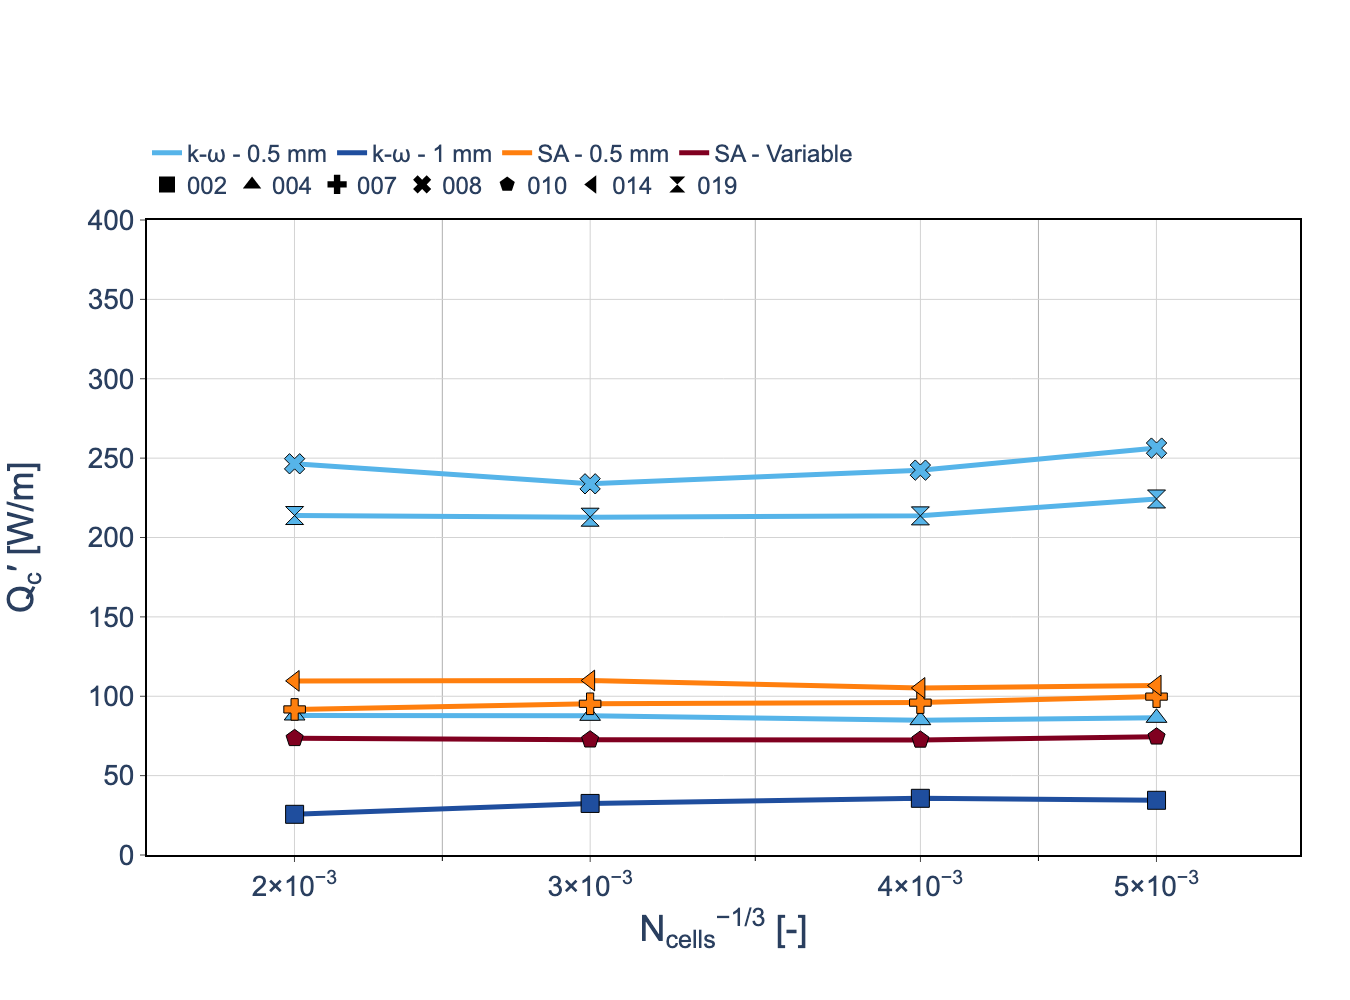
\includegraphics[trim={0cm 1cm 1cm 2.6cm}, clip, width=0.98\textwidth]{FIGURES/HTC/tc_naca0012_ae3933_qc_prime_vs_n_y_0.9144_grouped_turbulence_models.png}
    \textbf{AE3933}
\end{column}

\end{columns}
}

\centering
\textbf{Grouped by Turbulence Model / Roughness}
\vspace{-0.15cm}

\begin{block}{\scriptsize Observations}
\begin{itemize}
    \item<1-> $Q_c'$ shows limited grid sensitivity for most submissions.
    \item<2-> Grouping by turbulence model and roughness does not clearly explain the observed spread, as $Q_c$ also depends strongly on $T_s$ (and, to a lesser extent, $T_{rec}$) and on the HTC spread.
\end{itemize}
\end{block}

\end{frame}


% ============================================================
%  Surface Temperature
% ============================================================

\begin{frame}{\small  Surface Temperature Comparison (L1)}
\scriptsize
\vspace{-0.15cm}

% ------------------------------------------------------------
% All submissions
% ------------------------------------------------------------
\only<1>{
\begin{columns}[T,onlytextwidth]

\begin{column}{0.50\textwidth}
    \centering
    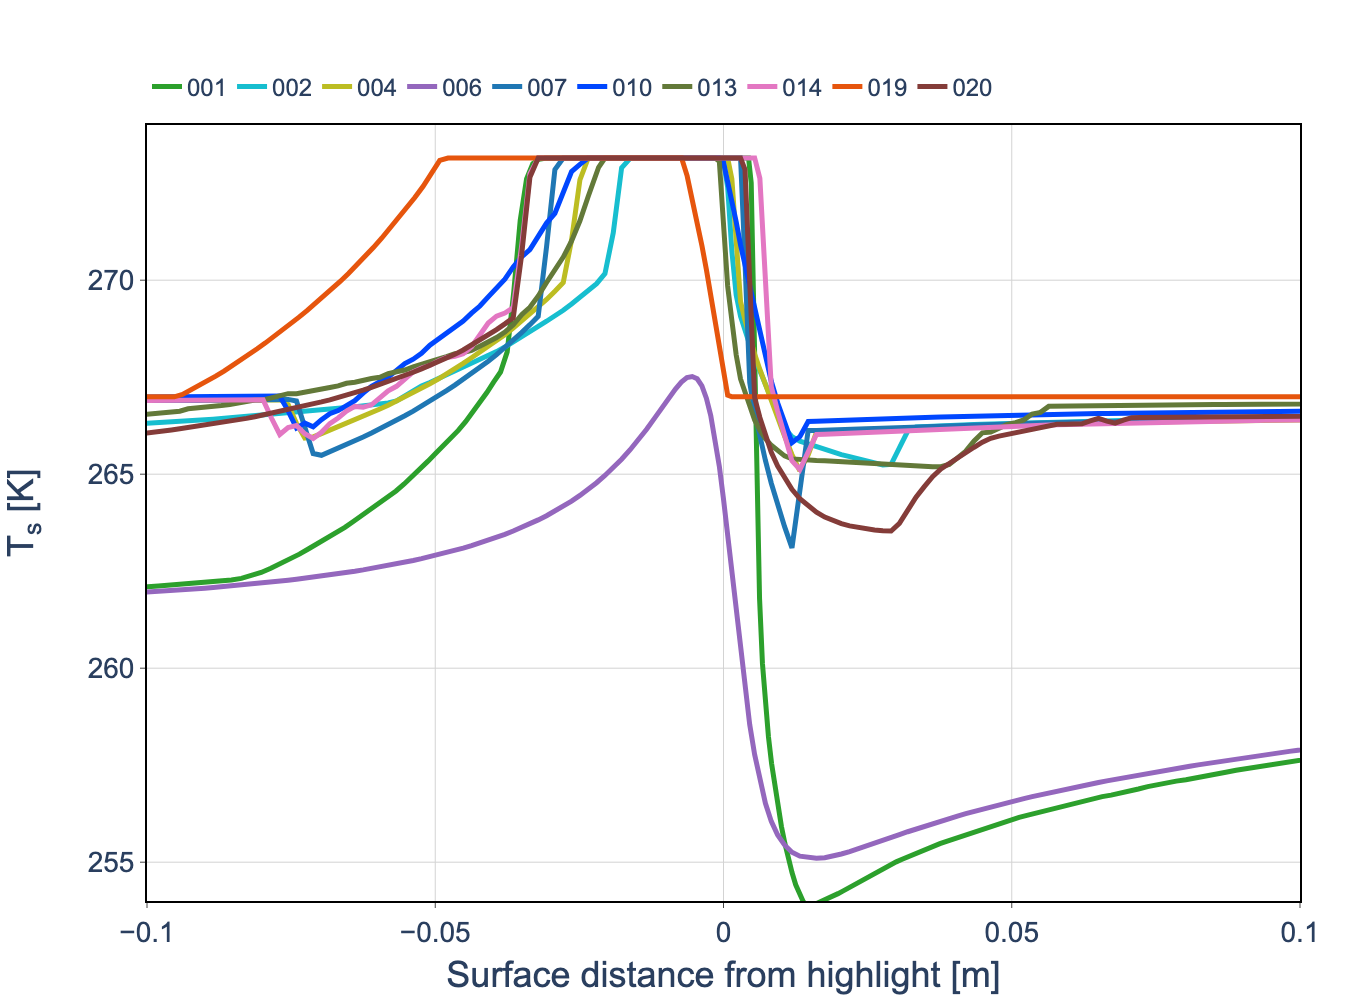
\includegraphics[trim={0cm 0cm 1cm 2.6cm}, clip, width=\textwidth]
    {FIGURES/SURF_TEMP_FF/tc_naca0012_ae3932_L1_surface_temperature_vs_s_slice_0p9144_all_roughness.png}

    {\scriptsize\textbf{AE3932}}
\end{column}

\begin{column}{0.50\textwidth}
    \centering
    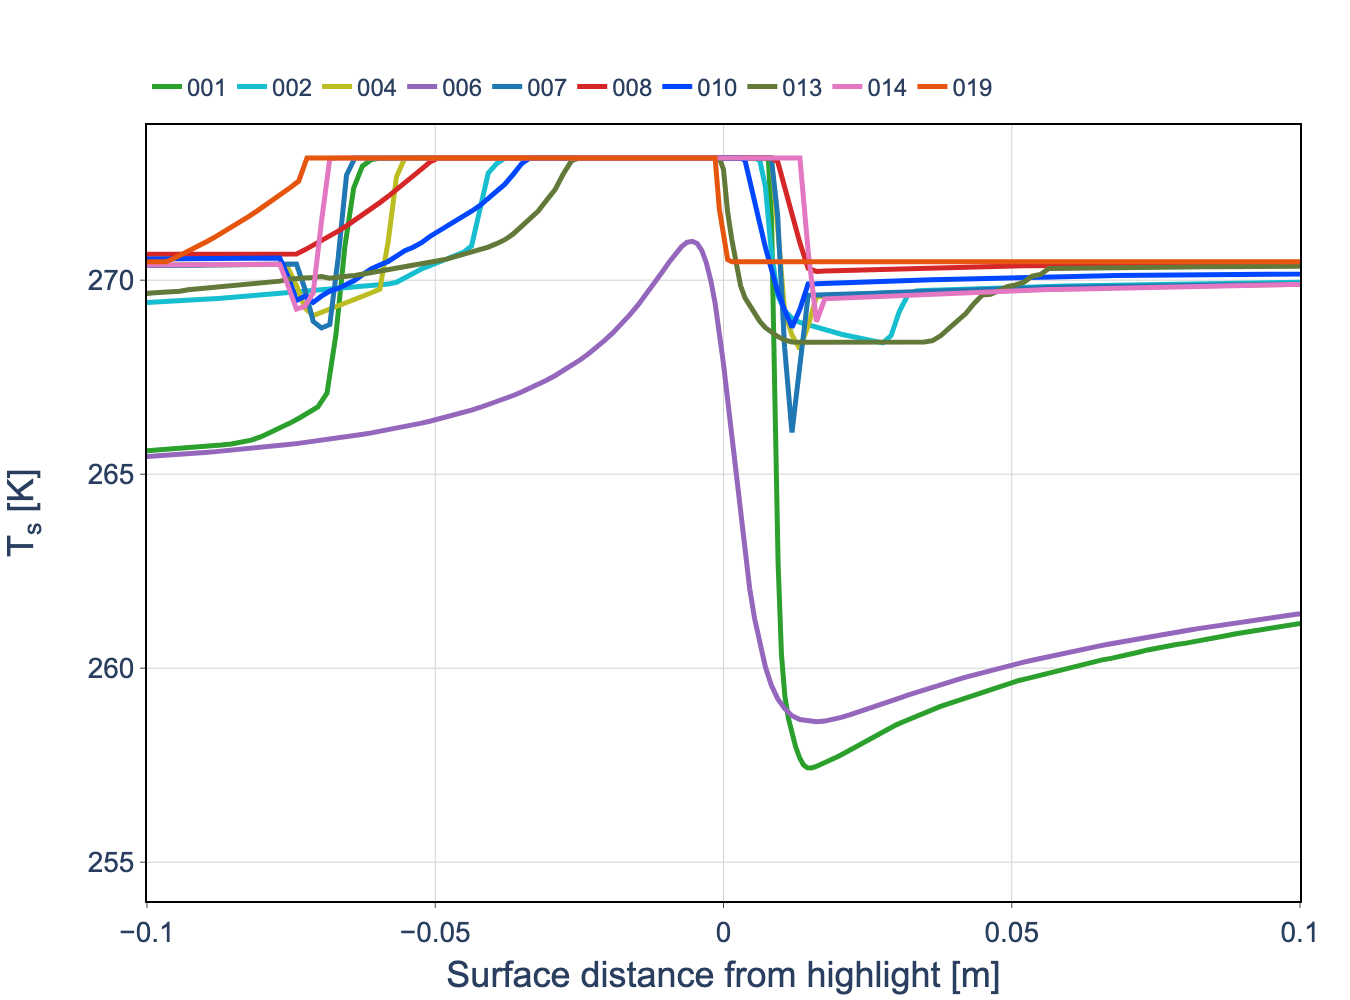
\includegraphics[trim={0cm 0cm 1cm 2.6cm}, clip, width=\textwidth]
    {FIGURES/SURF_TEMP_FF/tc_naca0012_ae3933_L1_surface_temperature_vs_s_slice_0p9144_all_roughness.png}

    {\scriptsize\textbf{AE3933}}
\end{column}

\end{columns}
}

% ------------------------------------------------------------
% Grouped by roughness
% ------------------------------------------------------------
\only<2>{
\begin{columns}[T,onlytextwidth]

\begin{column}{0.50\textwidth}
    \centering
    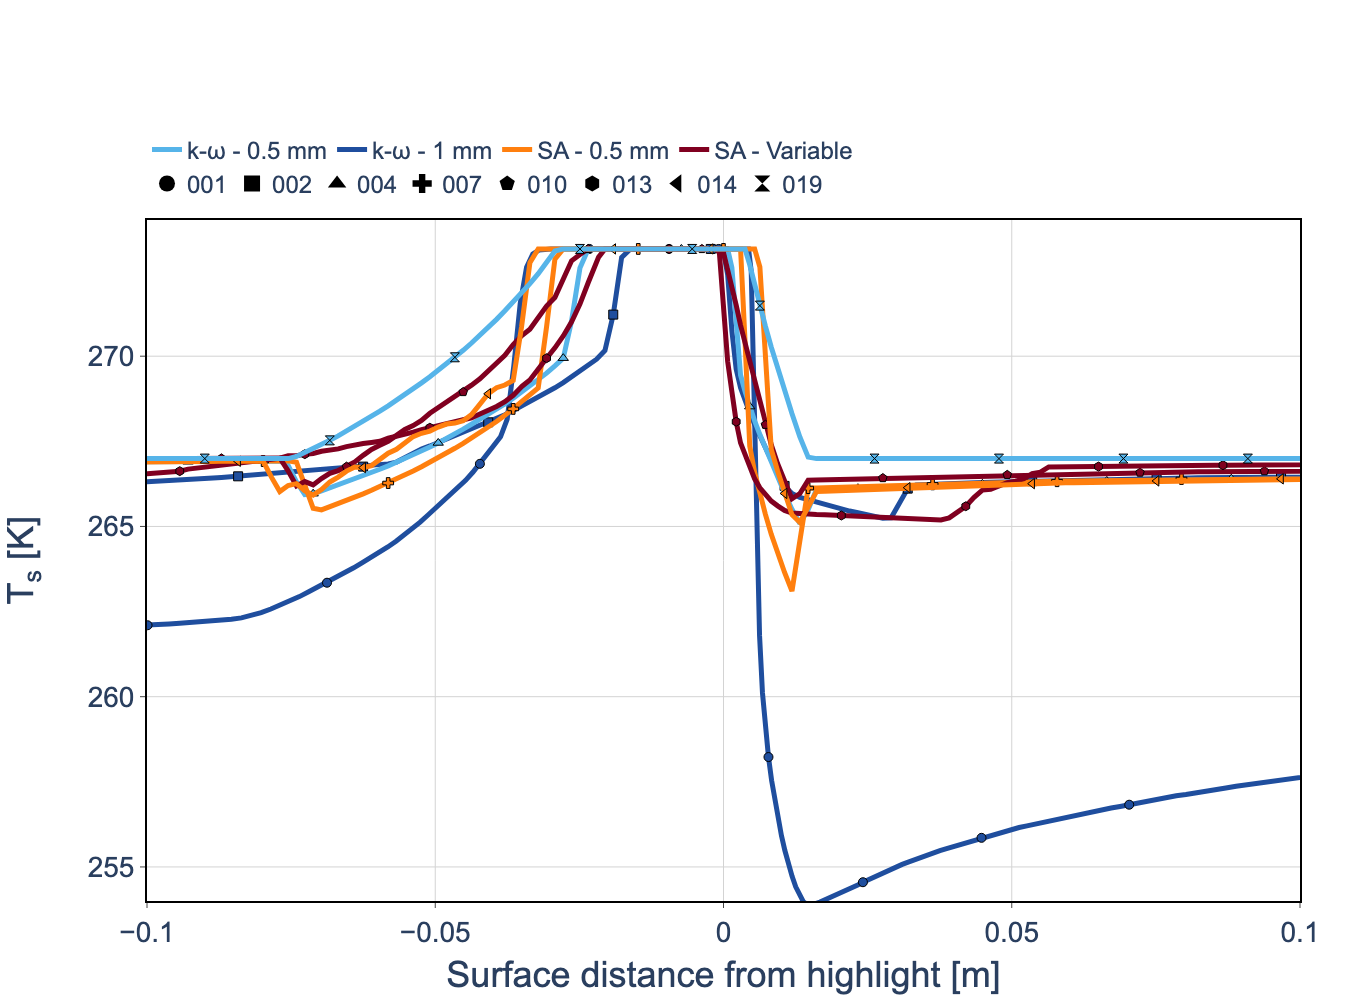
\includegraphics[trim={0cm 0cm 1cm 3.8cm}, clip, width=\textwidth]
    {FIGURES/SURF_TEMP_FF/tc_naca0012_ae3932_L1_surface_temperature_vs_s_slice_0p9144_grouped_turbulence_models.png}

    {\scriptsize\textbf{AE3932}}
\end{column}

\begin{column}{0.50\textwidth}
    \centering
    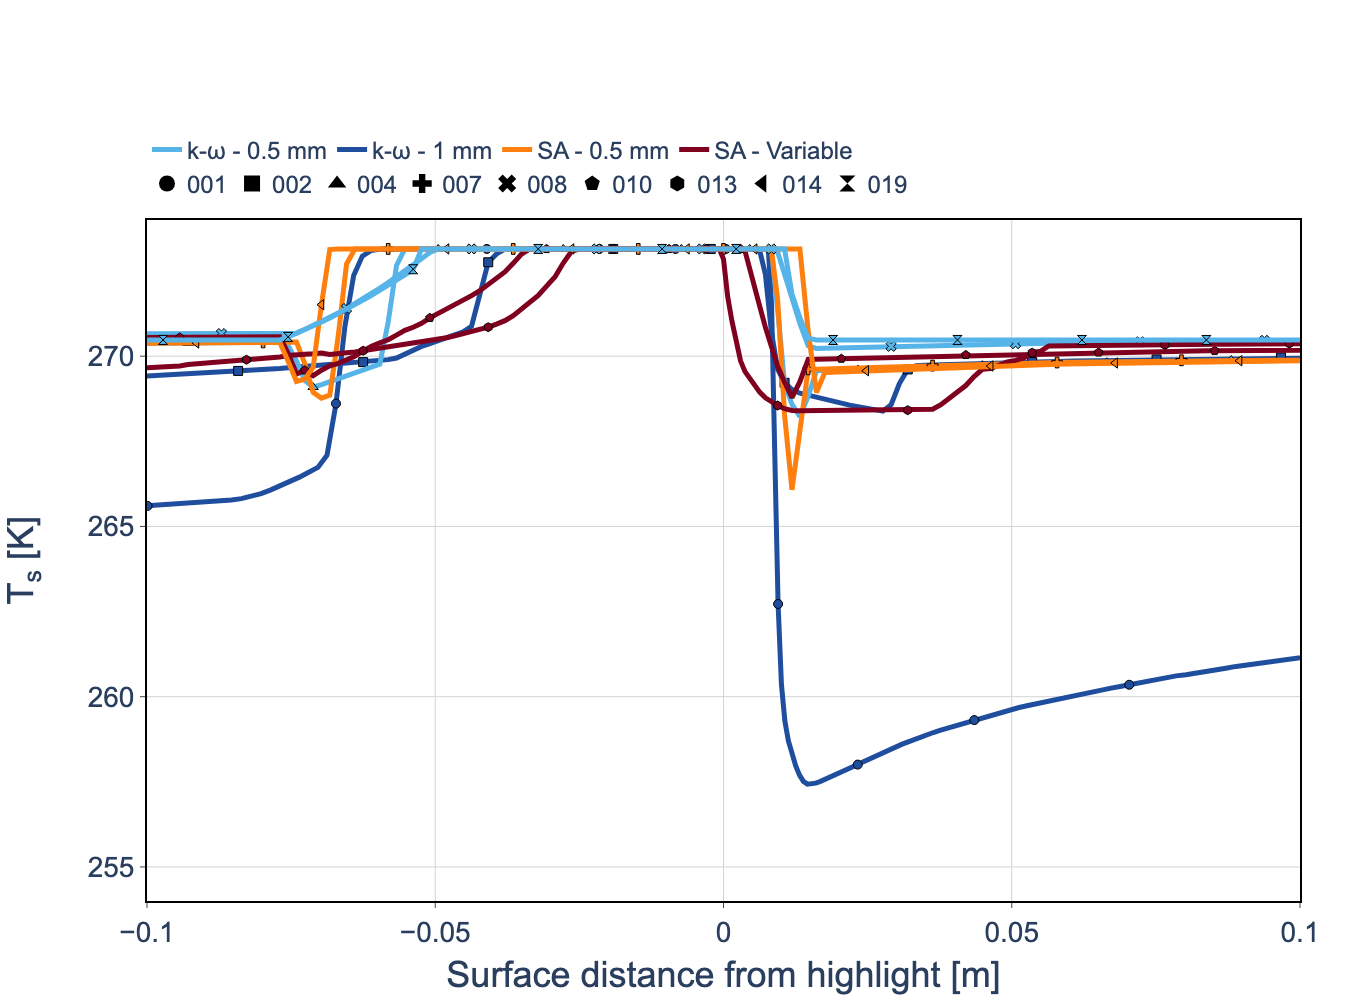
\includegraphics[trim={0cm 0cm 1cm 3.8cm}, clip, width=\textwidth]
    {FIGURES/SURF_TEMP_FF/tc_naca0012_ae3933_L1_surface_temperature_vs_s_slice_0p9144_grouped_turbulence_models.png}

    {\scriptsize\textbf{AE3933}}
\end{column}

\end{columns}
}
\vspace{-0.05cm}
\centering
\textbf{Grouped by Turbulence Model / Roughness}
\vspace{-0.15cm}

\begin{block}{\scriptsize Observations}
\begin{itemize}
    \item<1-> Surface temperature shows substantial code-to-code variability; AE3933 exhibits a broader near-freezing region.
    \item<2-> Grouping by turbulence model, roughness, or thermodynamic model (not shown) reveals no clear systematic trend.
\end{itemize}
\end{block}

\end{frame}


% ============================================================
%  Freezing Fraction
% ============================================================

\begin{frame}{\small  Freezing Fraction Comparison (L1)}
\scriptsize
\vspace{-0.15cm}

% ------------------------------------------------------------
% All submissions
% ------------------------------------------------------------
\only<1>{
\begin{columns}[T,onlytextwidth]

\begin{column}{0.50\textwidth}
    \centering
    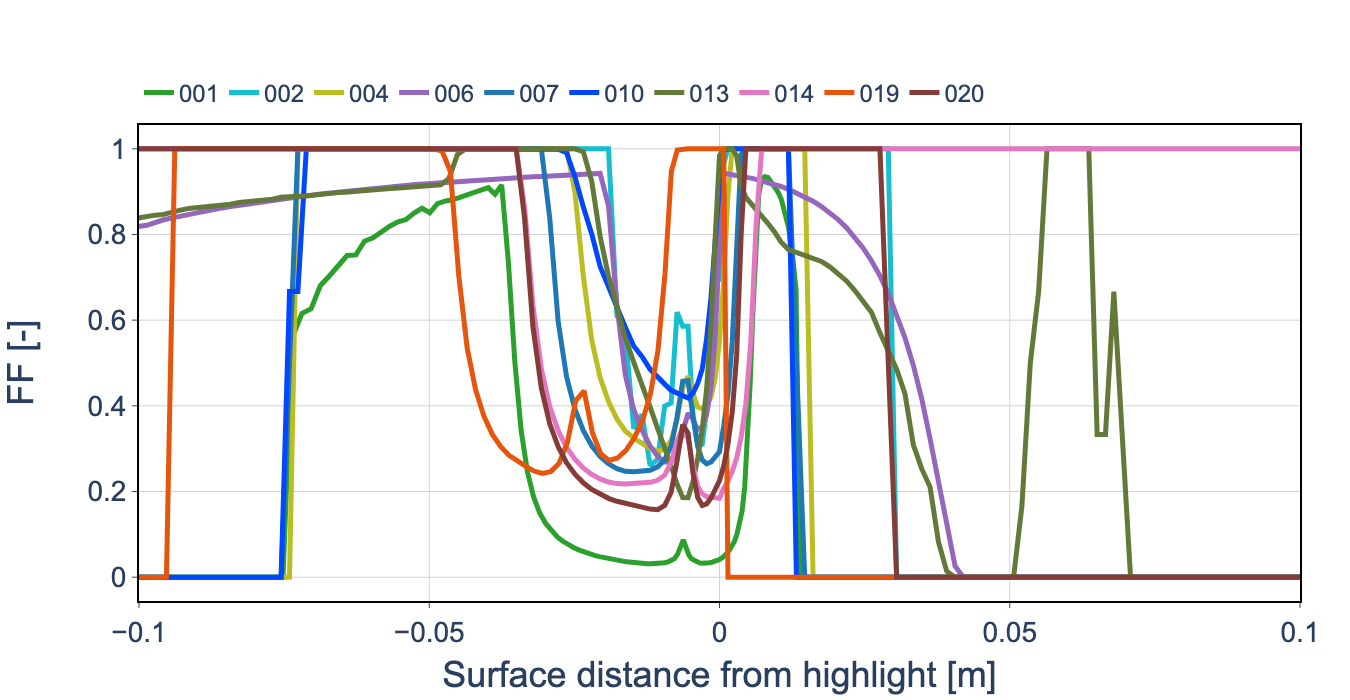
\includegraphics[trim={0cm 0cm 1cm 2.6cm}, clip, width=\textwidth]
    {FIGURES/SURF_TEMP_FF/tc_naca0012_ae3932_L1_freezing_fraction_vs_s_slice_0p9144_all_roughness.png}

    {\scriptsize\textbf{AE3932}}
\end{column}

\begin{column}{0.50\textwidth}
    \centering
    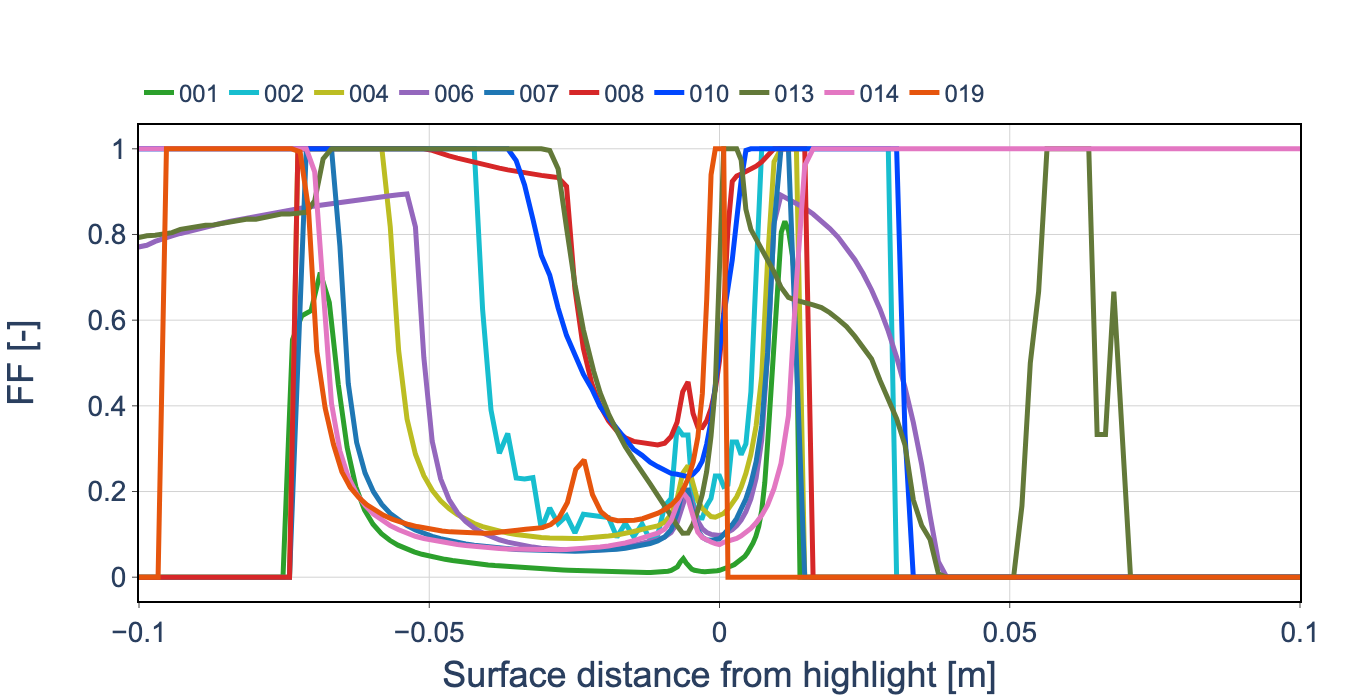
\includegraphics[trim={0cm 0cm 1cm 2.6cm}, clip, width=\textwidth]
    {FIGURES/SURF_TEMP_FF/tc_naca0012_ae3933_L1_freezing_fraction_vs_s_slice_0p9144_all_roughness.png}

    {\scriptsize\textbf{AE3933}}
\end{column}

\end{columns}
}

% ------------------------------------------------------------
% Grouped by roughness
% ------------------------------------------------------------
\only<2>{
\begin{columns}[T,onlytextwidth]

\begin{column}{0.50\textwidth}
    \centering
    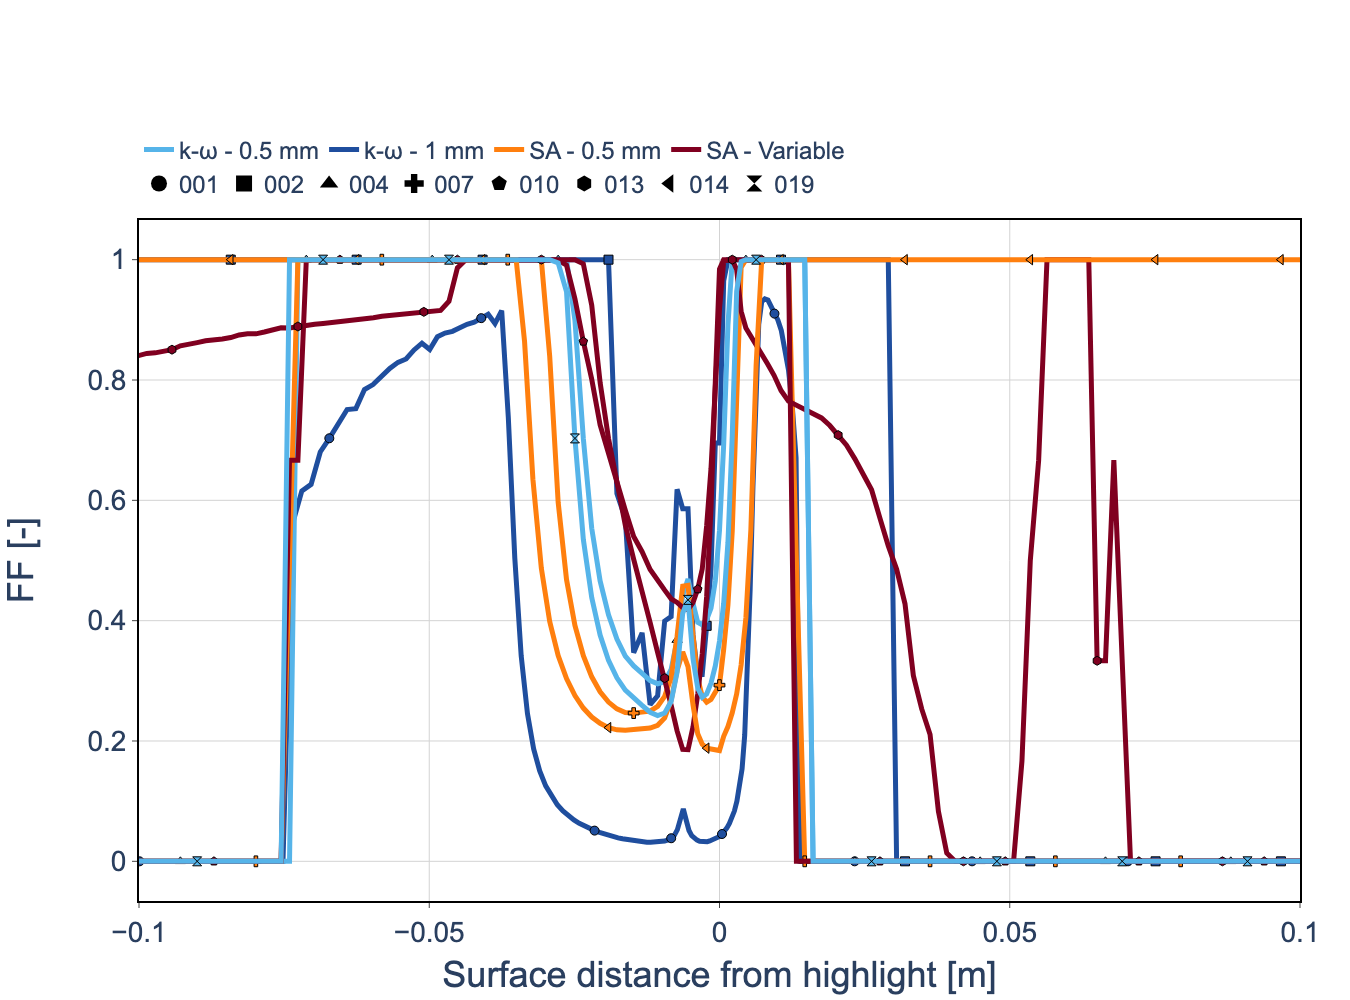
\includegraphics[trim={0cm 0cm 1cm 3.8cm}, clip, width=\textwidth]
    {FIGURES/SURF_TEMP_FF/tc_naca0012_ae3932_L1_freezing_fraction_vs_s_slice_0p9144_grouped_turbulence_models.png}

    {\scriptsize\textbf{AE3932}}
\end{column}

\begin{column}{0.50\textwidth}
    \centering
    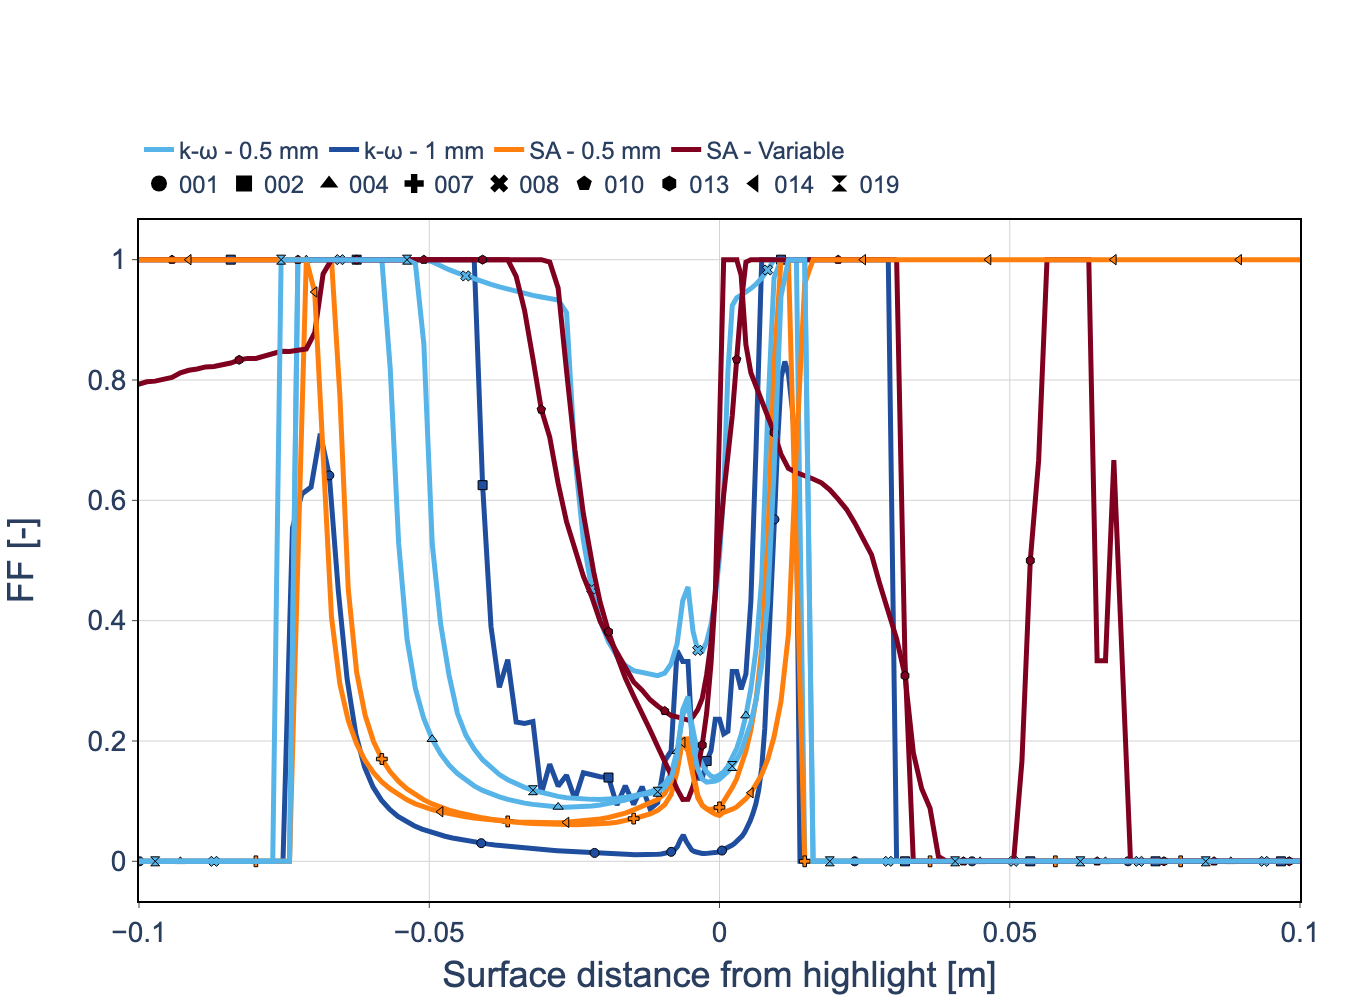
\includegraphics[trim={0cm 0cm 1cm 3.8cm}, clip, width=\textwidth]
    {FIGURES/SURF_TEMP_FF/tc_naca0012_ae3933_L1_freezing_fraction_vs_s_slice_0p9144_grouped_turbulence_models.png}

    {\scriptsize\textbf{AE3933}}
\end{column}

\end{columns}
}
\vspace{-0.1cm}
\centering
\textbf{Grouped by Turbulence Model / Roughness}

\vspace{-0.15cm}

\begin{block}{\scriptsize Observations}
\begin{itemize}
    \item<1-> Freezing fraction exhibits substantial code-to-code variability, with AE3933 showing a broader low-freezing-fraction region, consistent with its broader near-freezing surface-temperature region.
    \item<2-> Grouping by turbulence model, roughness, or thermodynamic model reveals no clear systematic similarities.
\end{itemize}
\end{block}

\end{frame}


% ============================================================
% HTC & Thermodynamics Assessment
% ============================================================

\begin{frame}{\small HTC \& Thermodynamics Assessment}
\scriptsize

\begin{alertblock}{\scriptsize HTC \& Thermodynamics Assessment}

\textbf{Convective Heat Transfer}
\begin{itemize}
    \item Local $HTC$ exhibits substantial code-to-code variability; turbulence modeling and roughness help explain the observed spread, while differences in $HTC$ computation methodology also play a role.
    
    \item Integrated convective heat transfer over the submitted data slice exhibits limited grid sensitivity for most submissions.
\end{itemize}

\vspace{0.10cm}

\textbf{Thermodynamic Response}
\begin{itemize}
    \item The code-to-code differences observed in $HTC$ are maintained in the surface temperature and freezing-fraction predictions, with no clear systematic trend when grouped by turbulence modeling or roughness height.
    
    \item The warmer AE3933 condition generally produces a wider near-freezing surface-temperature region and a correspondingly wider low-freezing-fraction region.
\end{itemize}

\end{alertblock}

\end{frame}